\documentclass{standalone}
\usepackage{tikz}

\usetikzlibrary{calc,intersections}


\begin{document}

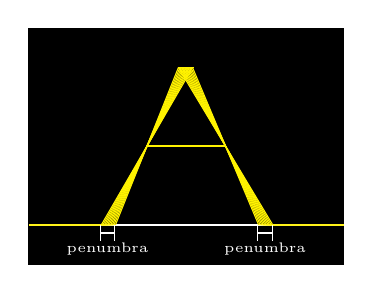
\begin{tikzpicture}
  \coordinate (L1) at (-0.1,2);
  \coordinate (L2) at (0.1,2);
  \coordinate (P1) at (-0.5,1);
  \coordinate (P2) at (0.5,1);

  \draw[fill=black] (-2,-0.5) rectangle (2,2.5);
  \draw[white!10,thick,name path=wall] (-2,0) -- (2,0);
  \draw[yellow,thick] (P1) -- (P2);
  \draw[yellow] (L1) -- (L2);

  \begin{scope}
    \path[clip] (-2,0) rectangle (2,2);

    \foreach \i in {0,0.1,...,1} {
      \coordinate (L) at ($ (L1) ! \i ! (L2) $);
      \draw[yellow]  (L) -- ($ (L) ! 2 ! (P1) $);
      \draw[yellow] (L) -- ($ (L) ! 2 ! (P2) $);
    }
  \end{scope}

  \foreach \i in {0,0.1,...,1} {
    \coordinate (L) at ($ (L1) ! \i ! (L2) $);
    \path[name path=ray1]  (L) -- ($ (L) ! 2 ! (P1) $);
    \path[name path=ray2] (L) -- ($ (L) ! 2 ! (P2) $);

    \draw[thick,yellow,opacity=0.2,,name intersections={of=wall and ray1,by=h1}] (-2,0) -- (h1);
    \draw[thick,yellow,opacity=0.2,name intersections={of=wall and ray2,by=h2}] (2,0) -- (h2);
  }

  \path[name path=ray1]  (L1) -- ($ (L1) ! 2 ! (P1) $);
  \path[name path=ray2]  (L2) -- ($ (L2) ! 2 ! (P1) $);
  \draw[|-|,white,name intersections={of=ray1 and wall,by=H1},name intersections={of=ray2 and wall,by=H2}] ($ (H1) + (0,-0.1) $) -- ($ (H2) + (0,-0.1) $) node[below,midway,font=\tiny] {penumbra};

  \path[name path=ray1]  (L1) -- ($ (L1) ! 2 ! (P2) $);
  \path[name path=ray2]  (L2) -- ($ (L2) ! 2 ! (P2) $);
  \draw[|-|,white,name intersections={of=ray1 and wall,by=H1},name intersections={of=ray2 and wall,by=H2}] ($ (H1) + (0,-0.1) $) -- ($ (H2) + (0,-0.1) $) node[below,midway,font=\tiny] {penumbra};
\end{tikzpicture}

\end{document}